\documentclass[runningheads]{llncs}
\usepackage[T1]{fontenc}
\usepackage{graphicx,amsmath,amssymb,booktabs,xcolor}
\usepackage[hidelinks]{hyperref}
\newcommand{\E}{\mathbb{E}}
\newcommand{\Var}{\operatorname{Var}}
\newcommand{\Cov}{\operatorname{Cov}}
\begin{document}
\title{Small Regions Look Homogeneous: Finite-Sample Bias of Radiomic Texture Features under Spatial Correlation, and When It Can Be Removed}
\titlerunning{Small Regions Look Homogeneous}
\author{Anonymous}
\authorrunning{Anonymous}
\institute{Anonymous institution}
\maketitle

\begin{abstract}
Radiomic texture features (entropy, uniformity, co-occurrence statistics) are computed inside a region of interest (ROI) and are known to depend on lesion volume. We show that a large part of this dependence is a statistical artefact with a predictable form, and we state when it can and cannot be removed. Modelling the image inside the ROI as a window onto a stationary random field, the plug-in bias of any smooth feature is $c/N$ for an ROI of $N$ voxels, with a constant $c$ fixed by the field's spatial correlation, so corrections that assume independent voxels under-correct. For quadratic features the bias has an exact closed form; for a quantised Gaussian field we compute it with Price's theorem and it matches simulation within Monte-Carlo error in 21 of 21 settings, with no fitted parameter. From the $c/N$ form we derive a delete-a-block jackknife that removes the bias without knowing $c$ and wraps any feature extractor unchanged. Importing fixed-domain asymptotics from geostatistics, we show why no ROI-based estimator can work when the ROI spans less than a few correlation lengths, and use the effective sample size $N/\xi^3$ as a per-ROI gate. On 6{,}560 real CT ROIs with an internal reference, including real reconstructions at 1.25--5\,mm, the gated jackknife removes the joint-entropy bias of 123-voxel ROIs ($-0.63\to-0.01$ bits), cuts its error by up to 59\%, and leaves test--retest repeatability unchanged.
\keywords{Radiomics \and Texture features \and Finite-sample bias \and Jackknife \and Identifiability}
\end{abstract}

\begin{figure}[t]\centering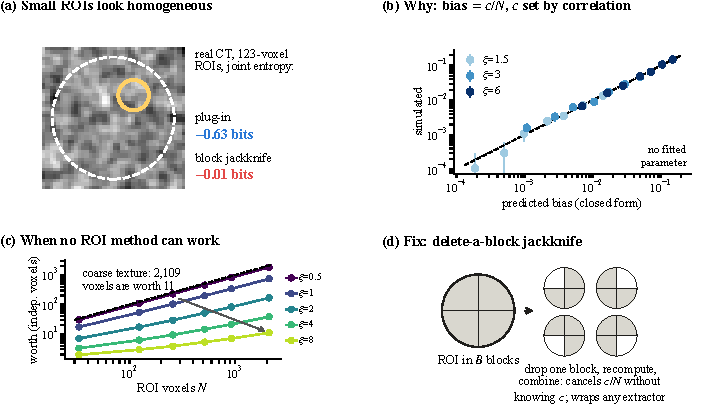
\includegraphics[width=\textwidth]{figures/fig_overview_ipmi.pdf}
\caption{\textbf{Overview.} (a) Texture features of small ROIs are biased: on real CT, the joint entropy of 123-voxel ROIs is 0.63 bits too low. (b) Modelling the ROI as a window onto a correlated random field gives the bias as $c/N$; for quadratic features the closed form matches simulation with no fitted parameter (uniformity shown; $\xi$: correlation length in voxels). (c) An ROI of $N$ correlated voxels carries the information of far fewer independent ones about the texture's scale (dashed: independent voxels), so below $N/\xi^3\approx20$ no ROI-based correction can work and the ROI is flagged. (d) Above that, a delete-a-block jackknife derived from the $c/N$ form removes the bias without knowing $c$.}\label{fig:overview}\end{figure}

\section{Introduction}
Radiomics summarises lesion heterogeneity with texture features computed inside a segmented ROI: first-order entropy and uniformity of the grey-level histogram and statistics of the grey-level co-occurrence matrix (GLCM)~\cite{haralick1973}, standardised by IBSI~\cite{zwanenburg2020} and implemented in PyRadiomics~\cite{vangriethuysen2017}. These \emph{plug-in} estimates are biased in small ROIs: the entropy of an under-sampled histogram is too low, so small lesions look homogeneous for purely statistical reasons. Volume confounding of radiomic features is well documented~\cite{welch2019}; Brooks and Grigsby~\cite{brooks2014} attributed it to under-sampling and proposed excluding lesions below a fixed volume, and Shafiq-ul-Hassan et al.~\cite{shafiq2017} proposed empirical normalisations. Classical entropy corrections, including Miller--Madow and the jackknife~\cite{miller1955,zahl1977,paninski2003}, assume independent samples, which neighbouring voxels are not. We found no general correction and no account of when a correction is possible at all.

\noindent\textbf{Problem.} Two questions are open (Fig.~\ref{fig:overview}). (Q1) What is the finite-sample bias of a texture feature computed on a spatially correlated image, and can it be predicted? (Q2) When can it be removed from the ROI alone, and when is no estimator able to do so?

\noindent\textbf{Contributions.} (i) \emph{Model} (Sec.~\ref{sec:model}): a stationary-field model of the ROI gives the bias of every smooth feature as $c/N$, with $c$ inflated by spatial correlation, and an exact closed form for quadratic features that we compute for quantised Gaussian fields with Price's theorem~\cite{price1958}; it predicts simulated bias with no fitted parameter. (ii) \emph{Identifiability} (Sec.~\ref{sec:ident}): importing fixed-domain asymptotics from geostatistics~\cite{zhang2004,stein1999}, an ROI smaller than a few correlation lengths carries almost no information about the texture's marginal scale, so no ROI-based correction can work there. (iii) \emph{Method} (Sec.~\ref{sec:method}): a delete-a-block jackknife derived from the $c/N$ form removes the bias without estimating $c$, gated per ROI by $N/\xi^3$. (iv) \emph{Evidence} (Sec.~\ref{sec:exp}): ground truth first (synthetic fields), then real CT with an internal reference, real reconstructions, all 93 non-shape PyRadiomics features and lung tumours.

\noindent\textbf{Scope and limits (stated up front).} The model assumes stationarity inside the ROI; real tumours are heterogeneous, so their size--feature relations mix bias and biology. The closed form is exact for quadratic features; for entropy, the second-order expansion over-predicts the bias by 40--50\% (Sec.~\ref{sec:res-theory}), which is why the method does not rely on it. The gate index $N/\xi^3$ is a proxy that overstates the effective sample size of very rough texture ($\xi<1$ voxel). Run- and zone-based features are outside the model.

\section{A model of the ROI and the bias it predicts}\label{sec:model}
\noindent\textbf{Setting.} Let $X$ be a stationary random field on $\mathbb{Z}^3$ and $S$ an ROI of $N$ voxels. A grey-level discretisation with bins $B_1,\dots,B_K$ maps each voxel to an indicator vector $e(X_s)\in\{0,1\}^K$; first-order features are functions $\theta=F(\pi)$ of the bin probabilities $\pi=\E\,e(X_0)$, GLCM features are functions of the joint probabilities of bin pairs at a fixed offset. The plug-in estimate is $\hat\theta_S=F(\hat\pi_S)$ with $\hat\pi_S=N^{-1}\sum_{s\in S}e(X_s)$.

\begin{proposition}[Bias under correlation]\label{prop:bias}
Let $C(h)=\Cov(e(X_0),e(X_h))$. Then $\Cov(\hat\pi_S)=N^{-2}\sum_{s,t\in S}C(t-s)$ exactly, and for $F$ twice differentiable,
\begin{equation}
\E\,\hat\theta_S-\theta=\tfrac12\operatorname{tr}\!\big(\nabla^2F(\pi)\,\Cov(\hat\pi_S)\big)+R_S,\label{eq:bias}
\end{equation}
with $R_S$ of third order in $\hat\pi_S-\pi$. If $\Sigma_\infty=\sum_h C(h)$ converges and $S$ grows with a vanishing boundary fraction, $\Cov(\hat\pi_S)=\Sigma_\infty/N+o(1/N)$, so the leading bias is $c/N$ with $c=\tfrac12\operatorname{tr}(\nabla^2F\,\Sigma_\infty)$.
\end{proposition}
\noindent For independent voxels $\Sigma_\infty=\operatorname{diag}\pi-\pi\pi^\top$ and, for entropy, \eqref{eq:bias} is the Miller--Madow bias $-(K-1)/(2N\ln2)$ bits~\cite{miller1955}. Under correlation, $\Sigma_\infty$ is inflated by the sum of the indicator autocovariances over all lags, roughly the correlation volume $\xi^3$ (a ``design effect''). The constant is unknown and image-dependent, so independent-sample corrections under-correct.

\begin{proposition}[Exact bias of quadratic features]\label{prop:quad}
For uniformity $U=\sum_k\pi_k^2$ (and any quadratic $F$, e.g.\ GLCM joint energy with pair indicators), $R_S=0$ and $\E\,\hat U_S-U=\sum_k\Var(\hat\pi_{S,k})$, which by Proposition~\ref{prop:bias} is a finite sum over the ROI's pair-offset histogram.
\end{proposition}
\noindent\emph{Proof.} $\E\hat\pi_{S,k}^2=\pi_k^2+\Var(\hat\pi_{S,k})$. \qed

\noindent\textbf{Closed form for a quantised Gaussian field.} If $X$ is Gaussian with correlation $\rho(h)$ and bin $k$ is the interval $(u_k,v_k)$ in standard units, then $C_{kk}(h)=P(X_0\in B_k,X_h\in B_k)-\pi_k^2$ is a function of $\rho(h)$ only. By Price's theorem~\cite{price1958}, $\partial P(X\le a,Y\le b)/\partial\rho=\varphi_2(a,b;\rho)$, hence
\begin{equation}
C_{kk}(\rho)=\int_0^{\rho}\big[\varphi_2(v_k,v_k;t)-2\varphi_2(u_k,v_k;t)+\varphi_2(u_k,u_k;t)\big]\,dt,\label{eq:price}
\end{equation}
a one-dimensional integral, exact at every $\rho$ including $\rho\to1$ (where a truncated Hermite series converges poorly). Together with the ROI's pair-offset counts (one FFT autocorrelation of the mask), Proposition~\ref{prop:quad} predicts the plug-in bias of uniformity for any ROI shape with no free parameter, and \eqref{eq:bias} gives the second-order prediction for entropy, $-\sum_k\Var(\hat\pi_{S,k})/(2\pi_k\ln2)$.

\section{When no ROI-based correction can work}\label{sec:ident}
Marginal features such as first-order entropy depend on the field's marginal scale $\sigma$ (and on its shape). An ROI that spans only a fraction of a correlation length sees a nearly smooth surface: it reveals the local level and gradient, whose joint law depends on $\sigma$ and the correlation length $\xi$ mainly through $\sigma/\xi$. This is the regime of fixed-domain (infill) asymptotics in geostatistics: for a Mat\'ern field, only the ``microergodic'' combination $\sigma^2/\xi^{2\nu}$ is consistently estimable within a bounded domain, and $\sigma$ and $\xi$ separately are not~\cite{zhang2004,stein1999}.

\begin{proposition}[Information about scale in a small ROI]\label{prop:ident}
For a Gaussian field with Mat\'ern correlation of length $\xi$ (unknown) and an ROI of fixed size relative to $\xi$, no estimator of $\sigma$, and hence of any marginal feature that varies with $\sigma$, is consistent as the voxel grid inside the ROI is refined~\cite{zhang2004}. Quantitatively, the efficient Fisher information about $\log\sigma$ with $\log\xi$ as nuisance is $I_{\sigma\sigma}-I_{\sigma\xi}^2/I_{\xi\xi}$ with $I_{ij}=\tfrac12\operatorname{tr}(\Sigma^{-1}\partial_i\Sigma\,\Sigma^{-1}\partial_j\Sigma)$, which we evaluate for spherical ROIs.
\end{proposition}
\noindent For ROIs with $N/\xi^3\le1$ this information is worth at most 3.9 (Mat\'ern $\nu=\tfrac12$) or 4.3 ($\nu=\tfrac32$) independent voxels, for ROIs of 33 to 2{,}109 voxels (Fig.~\ref{fig:theory}c); it grows only sublinearly with $N$ at fixed $\xi$. In this regime the bias is $O(1)$ rather than $O(1/N)$ and no correction based on the ROI alone can recover the population value; the right output is a flag. This motivates using the effective sample size $N/\xi^3$ as a per-ROI reliability index. It is a proxy: for $\xi<1$ voxel it exceeds $N$ and overstates the information (Fig.~\ref{fig:theory}c, $\xi=0.5$).

\section{Method: a block jackknife derived from the model}\label{sec:method}
Proposition~\ref{prop:bias} says the bias of a smooth feature is $c/|S'|$ for any contiguous region $S'$ much larger than $\xi$, with the \emph{same} unknown $c$. Split $S$ into $B$ contiguous blocks $S_b$ of $n_b$ voxels (we use $B=8$ octants at equal voxel quantiles along each axis) and recompute the feature on $S\setminus S_b$. The delete-a-group jackknife for unequal groups~\cite{busing1999},
\begin{equation}
\hat\theta_{\mathrm{JK}}=B\,\hat\theta_S-\textstyle\sum_{b}\big(1-\tfrac{n_b}{N}\big)\hat\theta_{S\setminus S_b},\label{eq:jk}
\end{equation}
then cancels the leading term for every $c$: if $\E\hat\theta_{S'}=\theta+c/|S'|$, the expectation of \eqref{eq:jk} is $B\theta+Bc/N-\sum_b(1-\tfrac{n_b}{N})(\theta+\tfrac{c}{N-n_b})=\theta$, since $\sum_b n_b=N$ and $(1-\tfrac{n_b}{N})/(N-n_b)=1/N$. Contiguity matters: deleting a contiguous block lowers the effective sample size in proportion to its voxel count, whereas deleting scattered voxels would not. The estimator needs $B+1=9$ calls of an unmodified extractor and no parameter; block resampling is classical for dependent data~\cite{kunsch1989,lahiri2003}, and we found no prior use for this problem.

\noindent\textbf{Gate.} We estimate $\xi$ inside the ROI as the lag at which the intensity autocorrelation falls to $1/e$ (mean over the three axes). The gated estimator returns $\hat\theta_{\mathrm{JK}}$ if $N/\xi^3\ge20$ and otherwise the plug-in value with an ``unreliable'' flag, since outside the $1/N$ regime the jackknife can add variance without removing bias, consistent with Proposition~\ref{prop:ident} and with the theory that a fixed number of subsamples cannot correct severely under-sampled entropies~\cite{jiao2020}.

\noindent\textbf{A second, non-statistical size artefact.} With a fixed bin width $w$, PyRadiomics numbers bins from the ROI minimum, $\lfloor x/w\rfloor-\lfloor x_{\min}/w\rfloor+1$. Features that use grey-level \emph{values} (GLCM joint/sum average, autocorrelation) then inherit the size dependence of an extreme-value statistic, which shrinks only logarithmically with $N$ and which no resampling can remove. Absolute bin indices $\lfloor x/w\rfloor$ (a fixed anchor) remove it.

\section{Experiments}\label{sec:exp}
\noindent\textbf{Ground truth: synthetic fields.} Gaussian random fields on $128^3$ grids (white noise filtered with a Gaussian kernel $\sigma\in\{0.75,1.5,3\}$ voxels, $\xi=2\sigma$, periodic boundary), scaled to CT-like intensities (mean 40, s.d.\ 60, bin width 25). For the theory test (preregistered, Sec.~\ref{sec:res-theory}) we draw 400 spherical ROIs per (field, radius) cell, radii 3--14 voxels (123--11{,}513 voxels), and compare the mean plug-in error with the analytic population value; the prediction uses the exact discrete correlation of the filter. For the jackknife we use 10 fields per $\sigma$ and a radius-60 reference sphere. Features come from a NumPy re-implementation of the PyRadiomics first-order and GLCM features that matches PyRadiomics~3.0.1 to five decimals.

\noindent\textbf{Real CT with an internal reference.} In the 63 CTs of the Medical Segmentation Decathlon lung task~\cite{antonelli2022} we place up to three spheres of radius 14 voxels (about 11{,}500 voxels) entirely inside soft tissue (HU in $[-50,150]$), giving 120 regions from 46 scans. Each large sphere is the reference; ROIs of radius 3--8 voxels are sampled inside it (1{,}045 ROIs; median $\xi=0.86$ voxels). To cover smoother textures we repeat this after Gaussian smoothing ($\sigma=0.7,1.4,2$; median $\xi=1.6,3.6,6.4$; 524, 499, 319 ROIs) and, with \emph{real} reconstructions, on RIDER Lung CT~\cite{zhao2024rider}: 32 patients scanned twice on the same day, each scan reconstructed with a sharp and a smooth kernel at 1.25, 2.5 and 5\,mm (251 series, 640 regions, 4{,}173 ROIs).

\noindent\textbf{All PyRadiomics features and lung tumours.} On 96 ROIs (radius 4 and 6, 29 scans) we wrap the unmodified PyRadiomics extractor (93 first-order, GLCM, GLRLM, GLSZM, GLDM and NGTDM features) in \eqref{eq:jk}; bias and RMSE are in units of the reference's between-region s.d. For the 66 MSD tumour components (68--338{,}472 voxels) we compute Spearman $\rho$ of each feature with volume, with and without correction, and on RIDER tumours (radiologist segmentations) the test--retest ICC(3,1).

\begin{figure}[t]
\centering
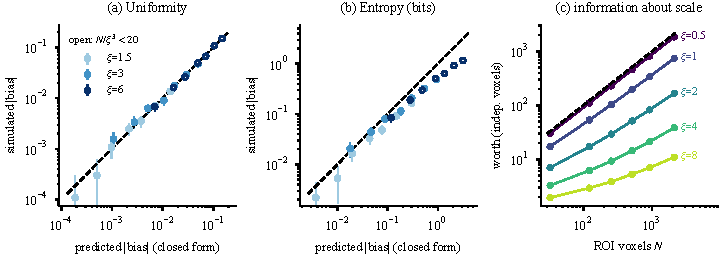
\includegraphics[width=\textwidth]{figures/fig_theory.pdf}
\caption{Theory against ground truth. (a,b) Predicted vs simulated plug-in bias (mean $\pm2$ s.e., 400 ROIs per point; open: $N/\xi^3<20$). Uniformity (exact, Prop.~\ref{prop:quad}) lies on the diagonal everywhere; the second-order entropy prediction overshoots. (c) Information about the texture scale in a spherical ROI when $\xi$ is unknown (Prop.~\ref{prop:ident}, Mat\'ern $\nu=\tfrac12$), in independent-voxel equivalents; dashed: independent voxels.}
\label{fig:theory}
\end{figure}

\section{Results}\label{sec:results}
\noindent\textbf{The model predicts the bias of quadratic features exactly (Fig.~\ref{fig:theory}a).}\label{sec:res-theory} We preregistered the comparison before running it. For uniformity the closed form matches the simulated bias within $\max(2\,\text{s.e.},10\%)$ in all 12 cells with $N/\xi^3\ge20$, and also in the small-ROI cells (e.g.\ $\xi=6$, $N=123$: predicted $0.1490$, simulated $0.1493\pm0.0048$), with no fitted parameter. For entropy the second-order expansion over-predicts by 40--50\% in every cell (median relative error 0.49; Fig.~\ref{fig:theory}b), so it fails the preregistered 20\% criterion. We note, without having tested it, that the expansion charges every rare tail bin about $1/N$ even when the ROI almost never fills it. A first, underpowered version of the same test (20 ROIs per cell, against a finite reference sphere) also failed its criterion. This is the reason the method uses the model only for its \emph{form} ($c/N$) and not for its constant.

\noindent\textbf{Small ROIs carry almost no information about the scale (Fig.~\ref{fig:theory}c).} The efficient information follows Proposition~\ref{prop:ident}: for $N/\xi^3\le1$ it is worth at most about four independent voxels. A preregistered check that it grows proportionally to $N/\xi^3$ failed (pooled log-log slope 0.64): for $\xi<1$ voxel, $N/\xi^3$ exceeds $N$, so the index overstates; at fixed $\xi\ge1$ growth is close to proportional.

\begin{figure}[t]
\centering
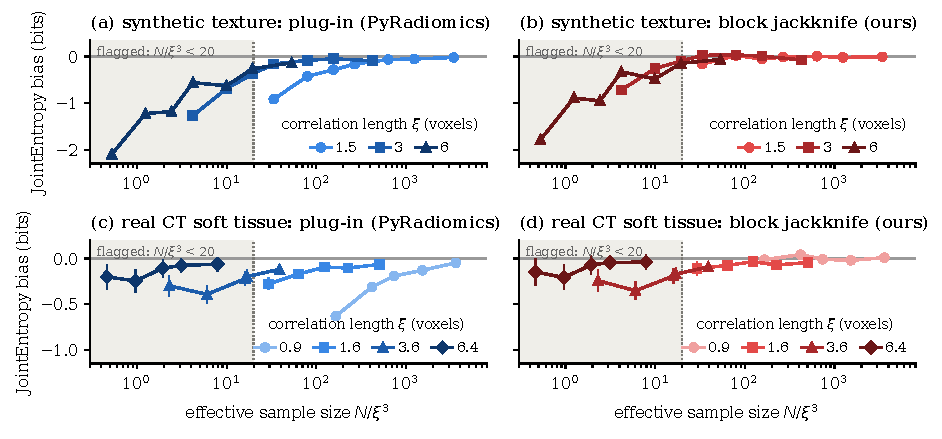
\includegraphics[width=\textwidth]{figures/fig_bias.pdf}
\caption{Bias of GLCM joint entropy vs effective sample size $N/\xi^3$, plug-in (a,c) vs block jackknife (b,d), on synthetic textures (a,b) and real CT soft tissue with an internal reference (c,d; mean and 95\% CI). One curve per correlation length (darker: longer); shaded: ROIs the gate flags.}
\label{fig:bias}
\end{figure}

\noindent\textbf{Synthetic textures (Fig.~\ref{fig:bias}a,b).} Plug-in joint entropy is biased by up to $-2.1$ bits and still by $-0.02$ to $-0.14$ bits at $11{,}500$ voxels. After correction the residual collapses onto one curve: it stays within $\pm0.1$ bits whenever $N/\xi^3\ge20$, for every correlation length. Below $N/\xi^3\approx5$ all estimators remain strongly biased, as Proposition~\ref{prop:ident} predicts. The correction raised the RMSE by more than $0.02$ only for contrast, which is unbiased.

\noindent\textbf{Real CT (Fig.~\ref{fig:bias}c,d).} In native soft tissue ($\xi=0.9$), a 123-voxel ROI underestimates joint entropy by $0.63$ bits; the jackknife removes this ($-0.01\pm0.05$, 95\% CI; over all radii bias $-0.27\to0.00$, RMSE $0.40\to0.23$). Smoother texture follows the gate: at $\xi=1.6$ the jackknife removes about half of the bias; at $\xi=3.6$ and $6.4$, where most ROIs have $N/\xi^3<20$, it removes little and can hurt (correlation: RMSE $0.36\to0.52$), which the gate prevents ($0.38$). Any threshold from 5 to 80 gives the same joint-entropy RMSE reduction (15\%). Real RIDER reconstructions confirm both regimes: with the sharp kernel at every slice thickness and the smooth kernel up to 2.5\,mm ($\xi\le1.1$; gate open for 96--100\% of ROIs) the jackknife removes 71--97\% of the joint-entropy bias (e.g.\ sharp, 1.25\,mm: $-0.34\to+0.03$ bits) and cuts the RMSE by up to 59\% ($0.46\to0.19$); with the smooth kernel at 5\,mm ($\xi=5.6$) the gate opens for only 32\% of ROIs. Across all 6 reconstructions gating never raised the RMSE of entropy, energy and uniformity features (${\le}0.1\%$); for nearly unbiased features (correlation, contrast, IDM) it raised it by up to 18\%, 5\% and 6\%.

\begin{figure}[t]
\centering
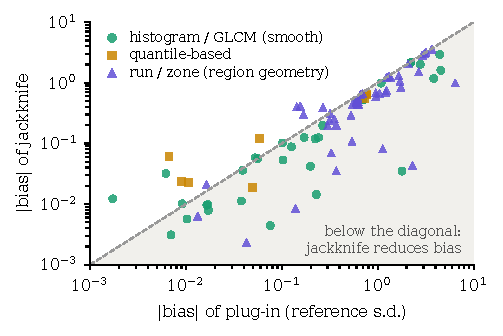
\includegraphics[width=0.62\textwidth]{figures/fig_pyrad.pdf}
\caption{Absolute bias of the 93 PyRadiomics features at radius 4 without (x) and with (y) the block jackknife.}
\label{fig:pyrad}
\end{figure}

\noindent\textbf{All PyRadiomics features (Fig.~\ref{fig:pyrad}).} 62 of 93 features are biased by more than $0.2$ reference s.d.\ at radius 4. For smooth first-order and GLCM features the jackknife reduces the median bias from $0.15$ to $0.06$ s.d., lowers the RMSE for 22 of 34 and never raises it by more than 10\% (e.g.\ GLCM MCC $+1.79\to-0.03$ s.d., joint entropy $-0.23\to-0.01$). The remaining large biases in this group are definitional: energy and total energy are extensive, and joint average, sum average and autocorrelation inherit the ROI-minimum anchoring, which shifts the mean grey-level index by $-5.5$ levels at radius 3 and still $-1.7$ at radius 14, whereas a fixed anchor is unbiased at every radius. Quantile features behave as jackknife theory predicts (no gain; RMSE up ${>}10\%$ for 3 of 8), and region-geometry features are only partly corrected (median bias $0.63\to0.48$; 35 of 51 improved, 12 worse).

\noindent\textbf{Lung tumours.} Most tumours are large and most features change little; where the bias is large, the correction removes the size dependence: the correlation of GLCM Imc1 with volume drops from $\rho=0.65$ to $0.01$, of joint entropy from $0.13$ to $-0.02$, and the number of region-geometry features with $|\rho|>0.3$ from 35 to 22. Repeatability is unchanged: on RIDER tumours the test--retest ICC of joint entropy is $0.973$ (plug-in) vs $0.974$ (gated), of entropy $0.963$ vs $0.963$ (correlation: $0.89$ vs $0.85$).

\section{Discussion}
The finite-sample bias of radiomic texture features is not an unstructured nuisance: a stationary-field model fixes its form ($c/N$), gives its exact value for quadratic features, and says where no correction is possible. The method uses only the form, which is why it works for features whose constant the model cannot predict (entropy, where the second-order constant is 40--50\% too large). The fixed-domain argument explains why fixed volume thresholds are the wrong unit: what matters is the number of correlation lengths an ROI spans, which depends on reconstruction kernel and slice thickness as much as on volume. Our recommendations: gated jackknife for entropy/energy-type first-order and GLCM features (not linear or quantile ones), a fixed bin anchor, and reporting $N/\xi^3$ per ROI. Runtime is about 1\,s per RIDER tumour.

\noindent\textbf{Limitations.} Stationarity inside the ROI is assumed; the gate is necessary rather than sufficient, since non-stationary texture also separates small ROIs from large ones. The closed form was validated on Gaussian fields only. $N/\xi^3$ is a proxy that overstates information for $\xi<1$ voxel; an index capped at $N$ was not tested. Run- and zone-based features need definitional rather than statistical fixes. Code will be released upon acceptance.

\bibliographystyle{splncs04}
\bibliography{refs}
\end{document}
